\begin{figure}[h]
    \centering
    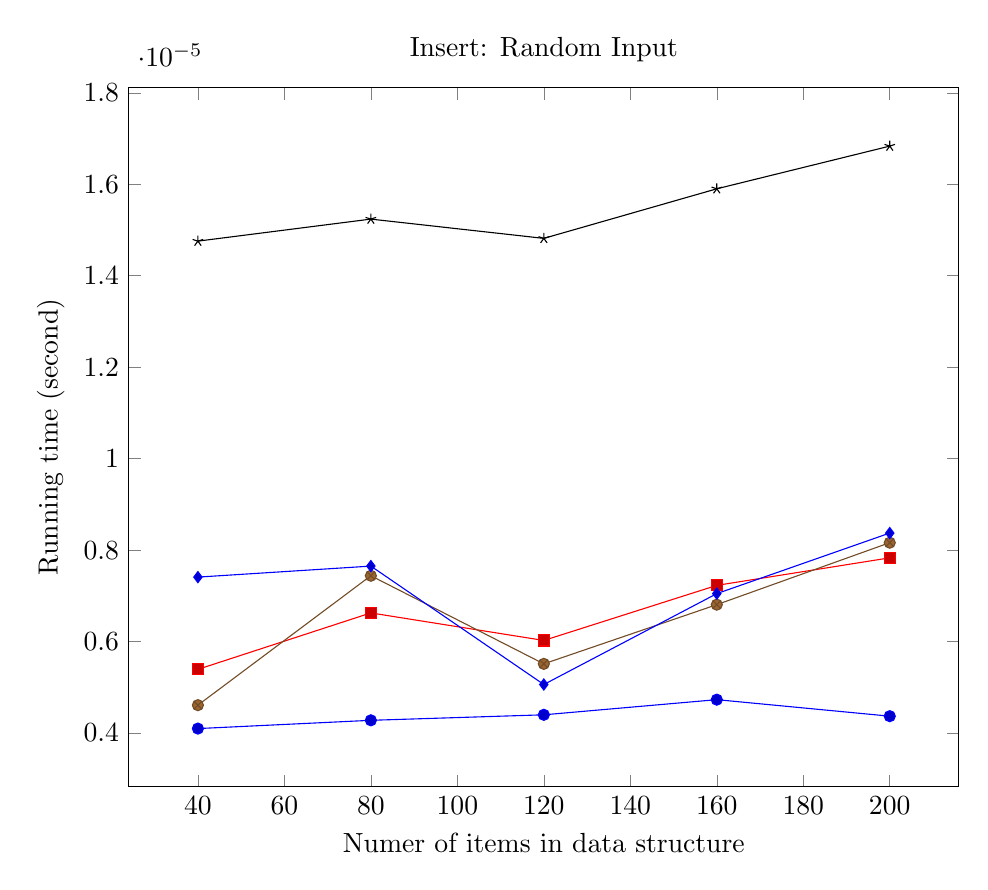
\begin{tikzpicture}
        \begin{axis}[
            xlabel={Numer of items in data structure},
            ylabel={Running time (second)},
            title={Insert: Random Input},
            width=\textwidth
        ]
		\addplot coordinates {
			(40, 4.095984580132494e-06)
			(80, 4.2766897816903794e-06)
			(120, 4.397159916535997e-06)
			(160, 4.728452787006176e-06)
			(200, 4.367042383179864e-06)
		};
		\addplot coordinates {
			(40, 5.391038527946534e-06)
			(80, 6.6258574086930365e-06)
			(120, 6.023506735175488e-06)
			(160, 7.228208082210585e-06)
			(200, 7.830558755372864e-06)
		};
		\addplot coordinates {
			(40, 4.607982652160558e-06)
			(80, 7.439030817835146e-06)
			(120, 5.511508662436882e-06)
			(160, 6.8065626102509215e-06)
			(200, 8.161851625843042e-06)
		};
		\addplot coordinates {
			(40, 1.4757591500824674e-05)
			(80, 1.5239472039496605e-05)
			(120, 1.4817826567892211e-05)
			(160, 1.590205778043696e-05)
			(200, 1.683570132442469e-05)
		};
		\addplot coordinates {
			(40, 7.408913284123741e-06)
			(80, 7.649853553459707e-06)
			(120, 5.059745657476355e-06)
			(160, 7.047502879942158e-06)
			(200, 8.372674361467603e-06)
		};
        \legend{}
        \end{axis}
    \end{tikzpicture}
    \caption{Average of 0 operations, benchmarked every 0, starting at 0.}
\end{figure}